% Section 5 - Consensus and Coordination (Habib Hasanov)
% Figure: ../diagrams/paxos_lwt.png (docs/diagrams/hasanov_diagrams.py)
% Measured values: \expsix{...}, \expfault{...} from generated/exp46_numbers.tex (analysis/summarize.py)
\providecommand{\expsix}[1]{\ifcsname expsix@#1\endcsname\csname expsix@#1\endcsname\else\textbf{[make exp6]}\fi}
\providecommand{\expfault}[1]{\ifcsname expfault@#1\endcsname\csname expfault@#1\endcsname\else\textbf{[make figures]}\fi}
\InputIfFileExists{generated/exp46_numbers.tex}{}{}

\section{Consensus and Coordination}\label{sec:consensus}

The assignment asks how the system elects leaders, replicates a log and prevents split-brain.
For Cassandra's ordinary reads and writes the precise answer is that \emph{it does none of
these}, and that is a design choice rather than an omission. Consensus appears in exactly one
place on the data path in 5.0---lightweight transactions---and arrives for metadata and
general transactions in 6.0.

\subsection{Ordinary operations: no leader, no log}

Any node can coordinate any request (Section~\ref{sec:consistency}). There is no primary
replica, no leader to elect and therefore no election timeout: when a node fails, requests are
simply coordinated by, and replicated to, the remaining nodes. Replicas do not share an ordered
log; each applies mutations in arrival order and order is recovered afterwards from
timestamps (Section~\ref{sec:antientropy}). Quorum replication is \emph{not} consensus: with
$R + W > N$ a read overlaps the latest acknowledged write, but two concurrent writers are
never ordered by agreement---both are acknowledged and LWW keeps one, and a timed-out write is
not rolled back. Experiment~6 makes this concrete: \expsix{plain-clients} clients inserting the
same handle with a plain QUORUM \texttt{INSERT} were all acknowledged, and
\expsix{plain-ackedoverwritten} acknowledged writes over \expsix{plain-handles} handles were
silently overwritten.

\paragraph{Gossip is dissemination, not agreement}
Membership, liveness, tokens and (up to 5.0) schema versions spread by gossip: every second
each node exchanges versioned state with one to three peers, so information reaches all
nodes in $O(\log n)$ rounds~\cite{demers1987epidemic}. Liveness is local opinion: the
$\varphi$-accrual detector~\cite{hayashibara2004phi} turns heartbeat inter-arrival times into a
suspicion level and marks a peer down above \texttt{phi\_convict\_threshold} (8). Different
nodes may hold different views at the same moment---exactly what a partition produces
(Section~\ref{sec:cap}). In our runs peers logged a killed node down after
\expfault{det-kill}\,s on average ($n=\expfault{det-kill-n}$), a partitioned node after
\expfault{det-part-majority}\,s, and a gracefully stopped node, which announces its shutdown,
after \expfault{det-stop}\,s. During the detection delay coordinators still believe the node is
alive, so ALL requests time out instead of failing fast with \texttt{Unavailable}.

\subsection{Lightweight transactions: Paxos per partition}

Conditional statements (\texttt{INSERT \ldots\ IF NOT EXISTS}, \texttt{UPDATE \ldots\ IF}) need
agreement: the check and the write must act on a single, agreed order of operations. Cassandra
runs single-decree Paxos~\cite{lamport1998parttime,lamport2001simple} among the replicas of the
\emph{one partition} being modified (Fig.~\ref{fig:paxos}). In the legacy implementation (v1,
the default in 5.0~\cite{cass21316}; our cluster ran \texttt{paxos\_variant =
\expsix{paxos-variant}}) a write takes four round trips:
(1)~\emph{prepare/promise}: the coordinator picks a ballot, a time-UUID higher than any it has
seen, and a majority of replicas promise to ignore lower ballots, returning any accepted but
uncommitted proposal, which must be completed first;
(2)~\emph{read}: the current row is read at quorum and the condition evaluated---if false, the
client receives \texttt{[applied] = False} together with the current values, and nothing is
proposed;
(3)~\emph{propose/accept}: the new value is accepted by a majority unless a higher ballot was
promised meanwhile;
(4)~\emph{commit}: the value is applied through the normal write path at the statement's
consistency level. The serial level of phases 1--3 is SERIAL (majority of all replicas) or
LOCAL\_SERIAL (majority in the local DC); a \texttt{SELECT} at SERIAL also completes any
in-flight proposal, giving linearizable reads~\cite{herlihy1990linearizability}.

There is no stable leader (Multi-Paxos, Raft~\cite{ongaro2014raft}): every LWT is a fresh
instance decided by ballots. Contention therefore costs retries---a proposer pre-empted by a
higher ballot restarts---and can end in \texttt{WriteTimeout} with write type CAS, whose
outcome is \emph{unknown}, not failed; our race classifier counts such ``timed-out winners''
explicitly. Paxos v2 (CEP-14~\cite{cep14}, opt-in since 4.1) reduces an uncontended write to
two round trips by merging the read into the prepare phase, and replaces the TTL-based cleanup
of Paxos state with Paxos repair. Guarantees remain per partition: there are no multi-partition
LWTs, and mixing LWT and non-LWT writes on the same cells voids linearizability because plain
writes bypass the ballots.

\begin{figure}[t]\centering
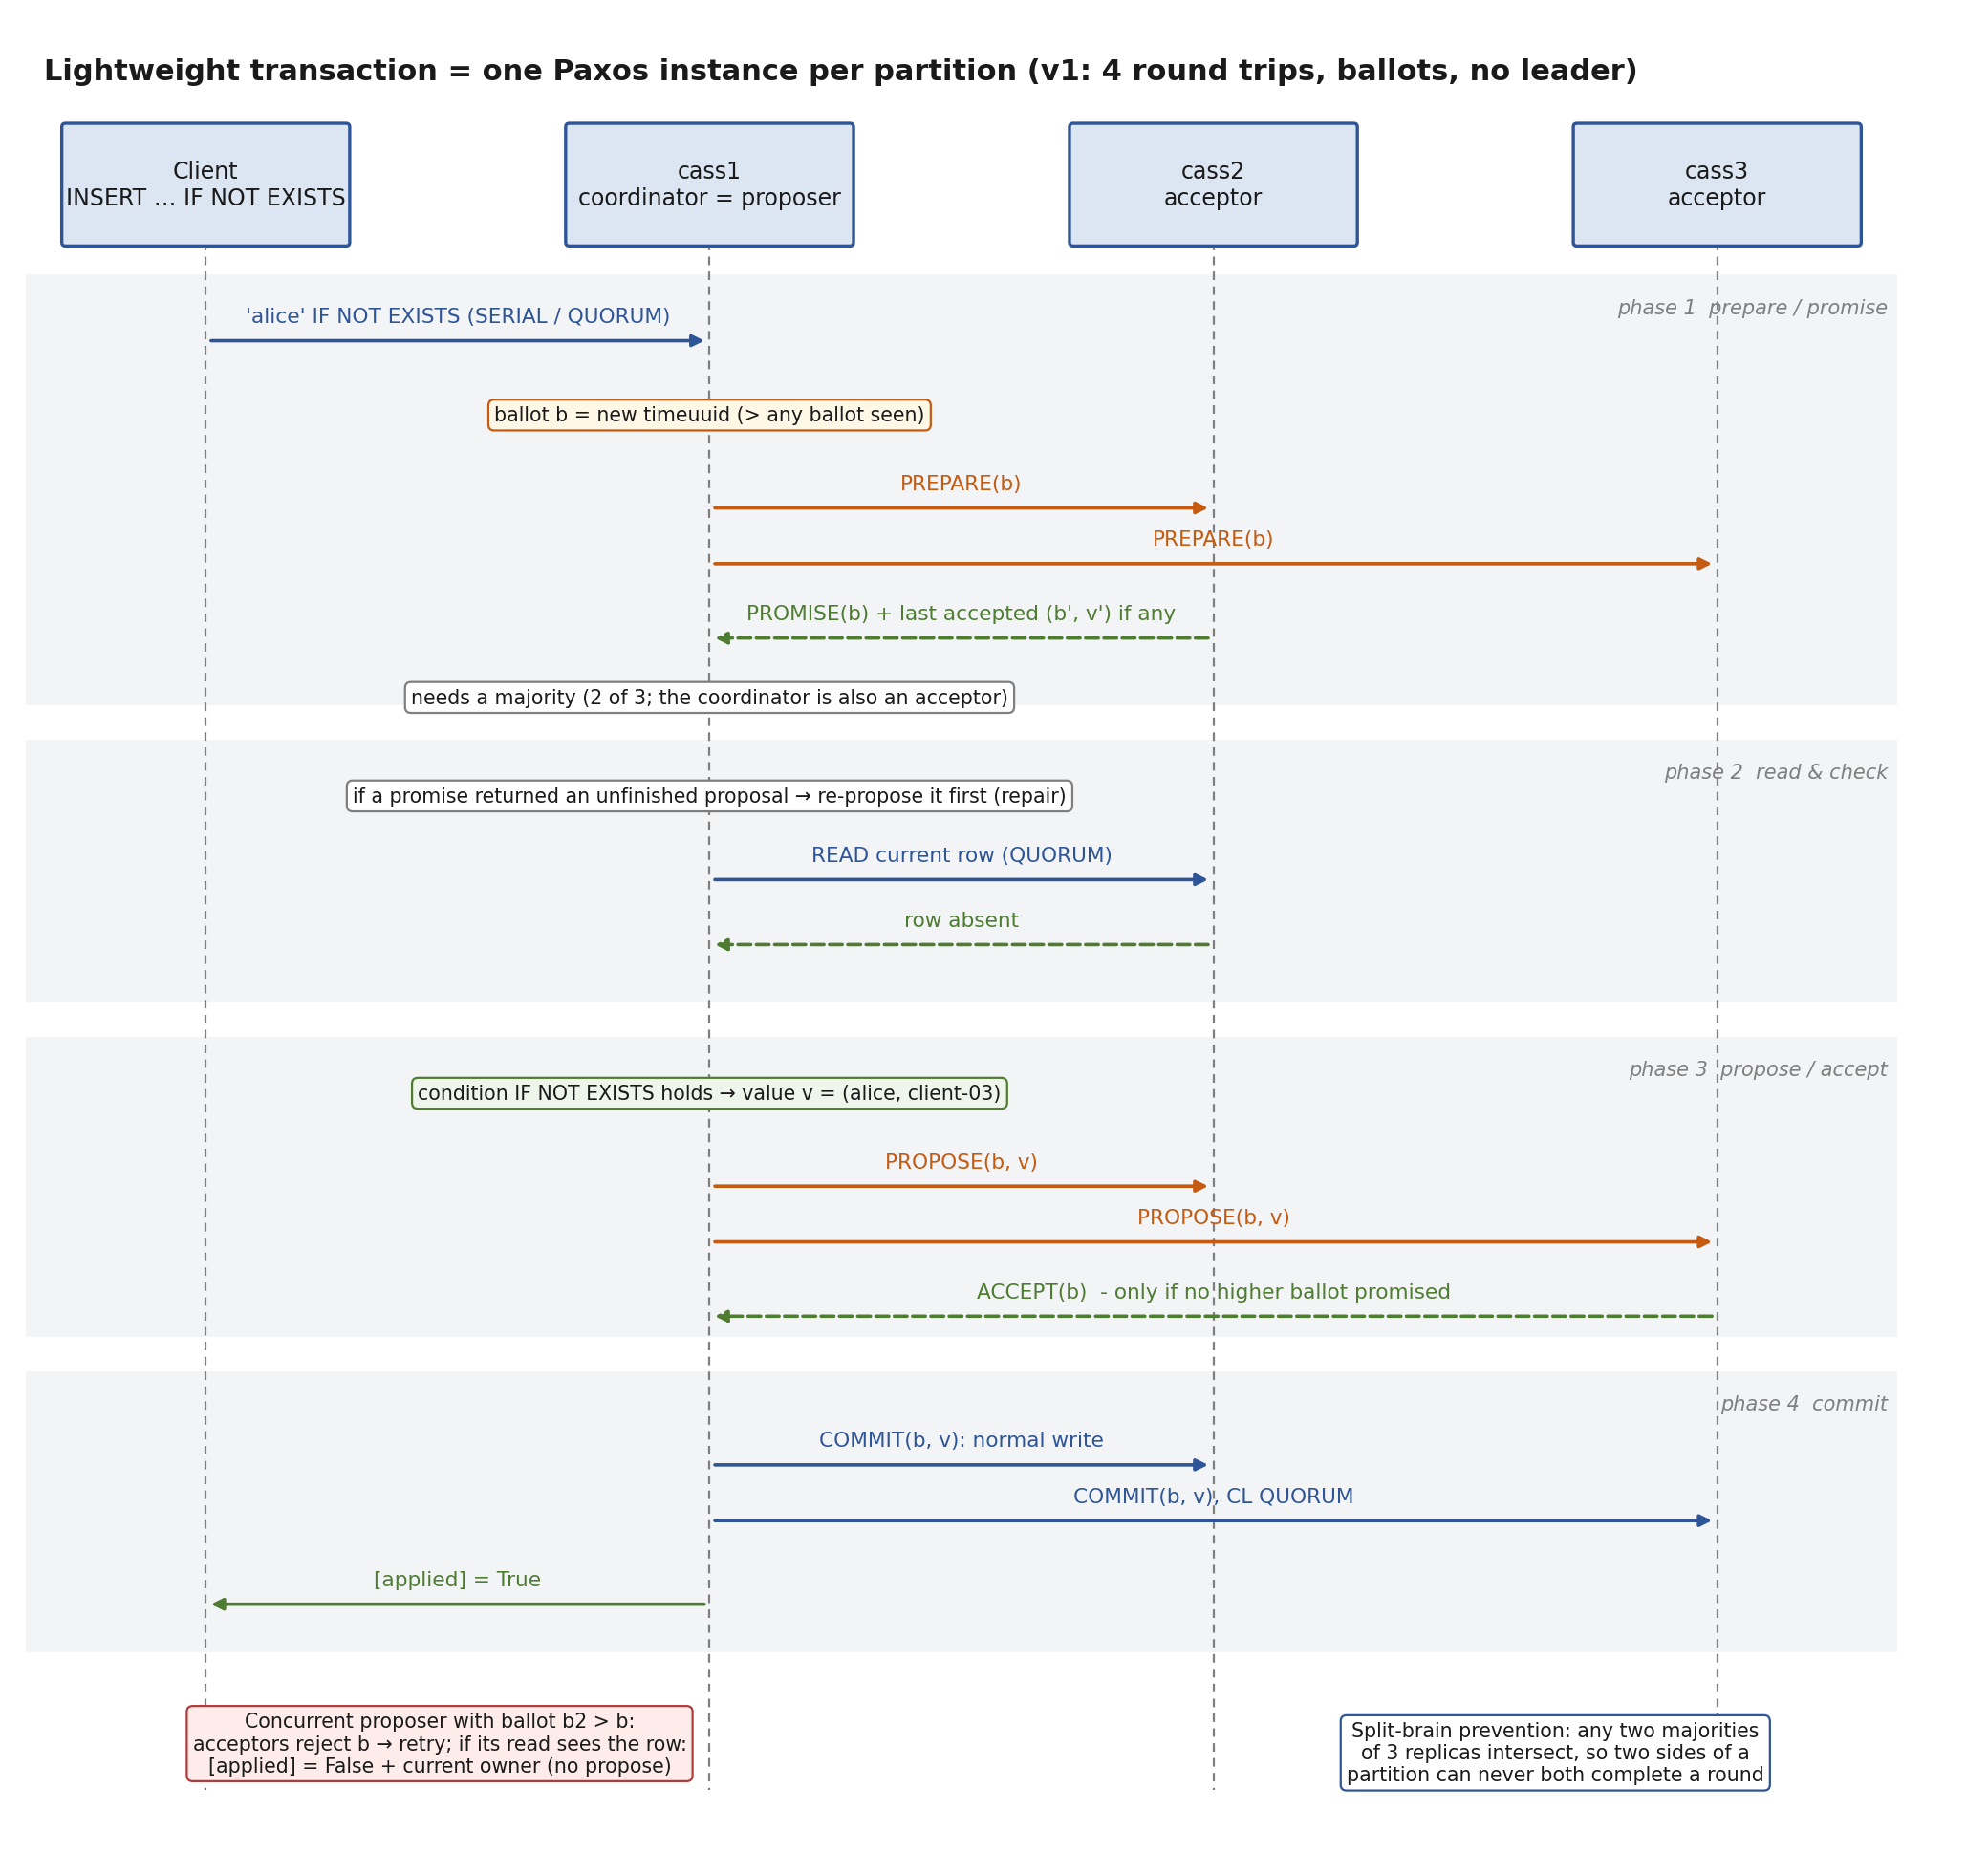
\includegraphics[width=\columnwidth]{paxos_lwt.png}
\caption{One Paxos v1 round of \texttt{INSERT \ldots\ IF NOT EXISTS} on a three-replica
partition; the coordinator is proposer and acceptor. A second proposer loses by ballot order or
sees the row in its read phase.}\label{fig:paxos}
\end{figure}

\subsection{Split-brain prevention}

Any two majorities of $N$ replicas intersect. A Paxos round needs a majority in both the
prepare and the accept phase, so the two sides of a partition can never both complete a round
for the same partition key: the minority side receives \texttt{Unavailable} or a timeout.
With $N = 3$, LWTs survive one failed replica and stop with two---Experiment~6 tests both
cases. Ordinary writes behave differently: at ONE \emph{both} sides of a partition accept
writes, and the divergence is resolved afterwards by LWW (Experiment~5). Cassandra thus does
not prevent split-brain for ordinary data; it tolerates it and reconciles deterministically,
which is what makes it available under partition~\cite{gilbert2002cap,abadi2012pacelc}.
Clients obtain split-brain-free behaviour per operation, by choosing QUORUM/SERIAL.

\subsection{Metadata coordination: gossip (5.0) and TCM (6.0)}

Up to 5.0, schema changes and token ownership also propagate by gossip. A schema change is
applied on one node and spreads as a schema version; nodes can disagree temporarily
(visible in \texttt{nodetool describecluster}---our schema script waits for one version), and
concurrent schema or topology changes can conflict. Cassandra 6.0 replaces this with
Transactional Cluster Metadata (CEP-21~\cite{cep21}): a Cluster Metadata Service keeps a
linearizable, epoch-numbered log of membership, ownership and schema transformations, and
nodes apply entries in log order, so topology changes become multi-step, committed sequences.
6.0 also introduces Accord (CEP-15~\cite{cep15,accord2021}), a leaderless protocol for
multi-partition transactions with strict-serializable isolation that can replace Paxos for
LWTs on migrated tables. At the time of writing 6.0 is a pre-release (6.0-alpha1, a
quarterly alpha for testing only~\cite{cass6alpha}); our measurements describe 5.0 as deployed.

\begin{table}[t]\centering\footnotesize
\setlength{\tabcolsep}{3pt}\caption{Coordination mechanisms and what they guarantee.}\label{tab:coordination}
\begin{tabular}{@{}p{0.26\columnwidth}p{0.2\columnwidth}p{0.16\columnwidth}p{0.25\columnwidth}@{}}\hline
Mechanism & Agreement & Leader & Tolerates ($N=3$) \\ \hline
Gossip / $\varphi$ detector & no (eventual) & none & any failures; views differ \\
Quorum read/write & no (LWW) & none & 1 failure at QUORUM \\
Paxos LWT (5.0) & yes, per partition & none (ballots) & 1 failure \\
TCM / CMS (6.0) & yes, global log & CMS members & minority of CMS \\
Accord (6.0) & yes, multi-partition & none & minority of replicas \\ \hline
\end{tabular}
\end{table}
